\chapter{VLANs: Part 3}\label{vlans-part-3}

\section{Native VLAN on a Router
(ROAS)}\label{native-vlan-on-a-router-roas}

\begin{figure}
\centering
\pandocbounded{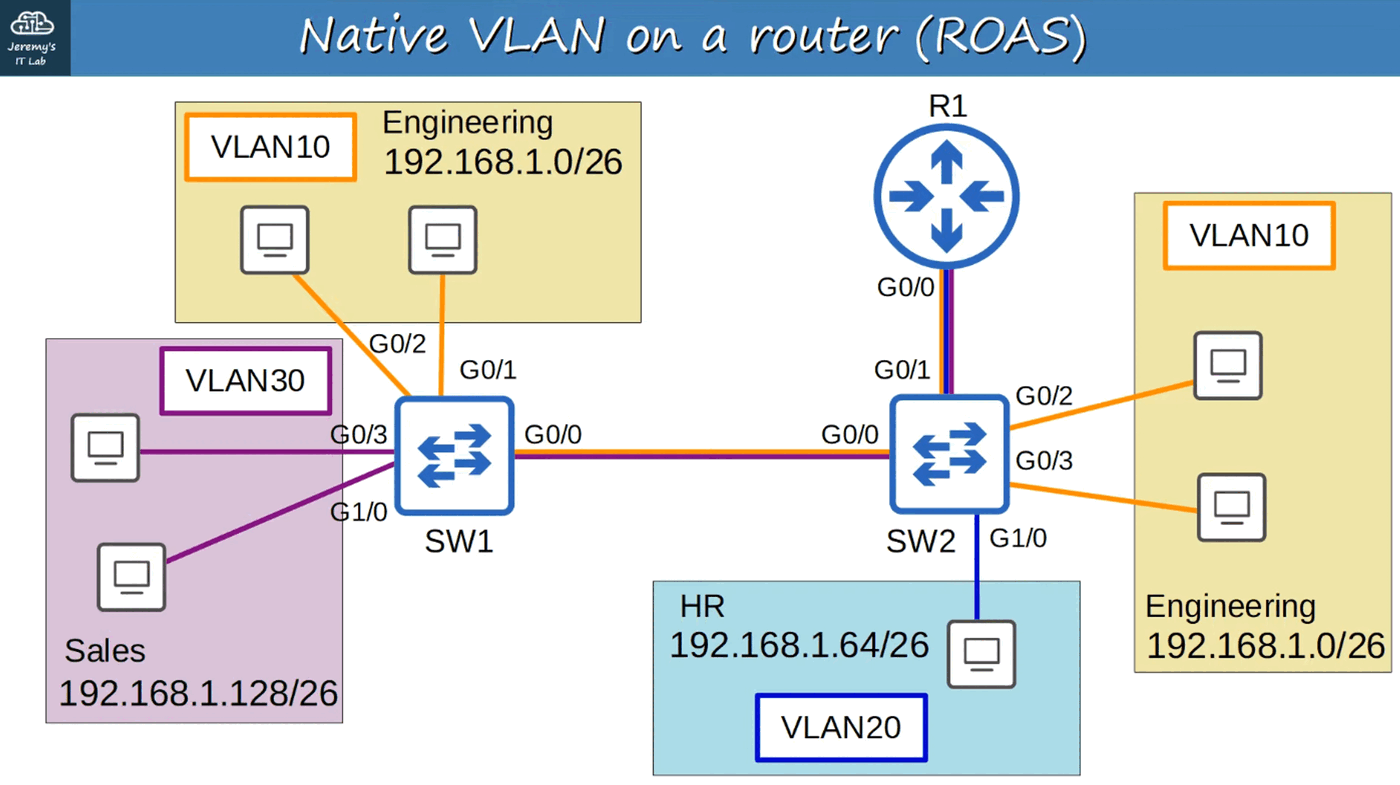
\includegraphics[keepaspectratio,alt={image}]{images/19-vlan-part3/img-001.png}}
\end{figure}

Native VLAN untagged frames are faster and more efficient (smaller) than
tagged ones.

Let's reset all SWITCHES (SW1 and SW2) to native vlan 10

\begin{figure}
\centering
\pandocbounded{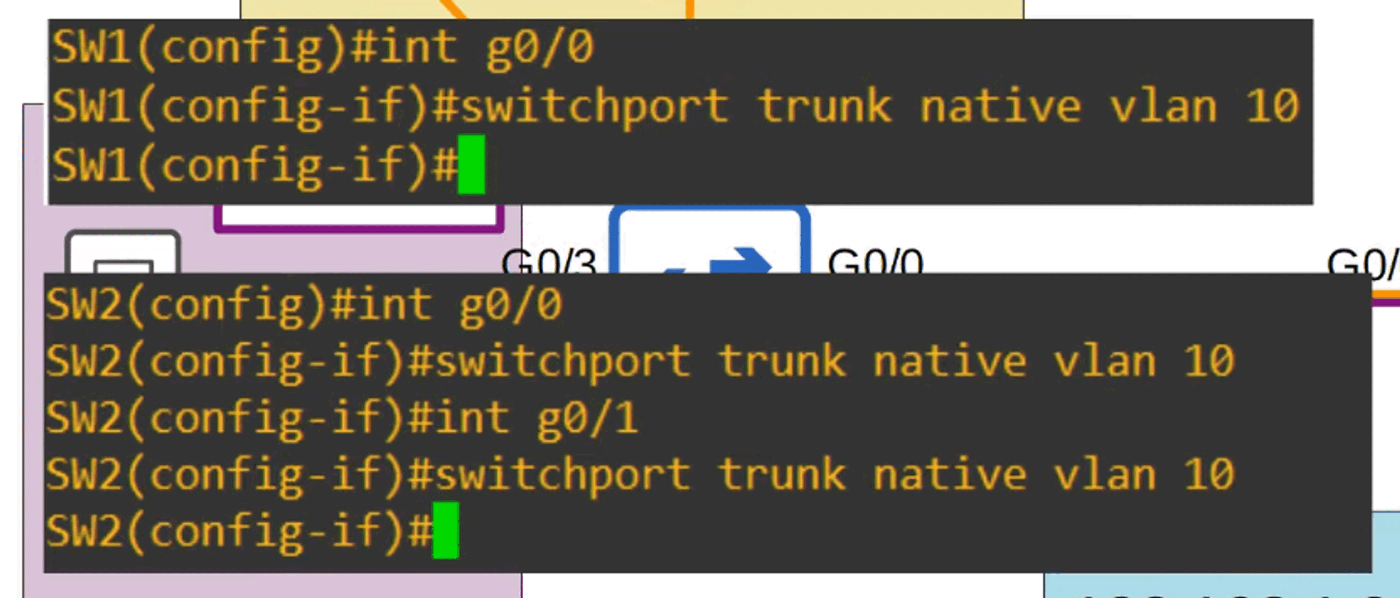
\includegraphics[keepaspectratio,alt={image}]{images/19-vlan-part3/img-002.png}}
\end{figure}

There are \textbf{TWO methods} of configuring the native VLAN on a
router:

\begin{itemize}
\tightlist
\item
  Use the command ``encapsulation dot1q \textless vlan-id\textgreater''
  on a Sub-Interface
\end{itemize}

\begin{figure}
\centering
\pandocbounded{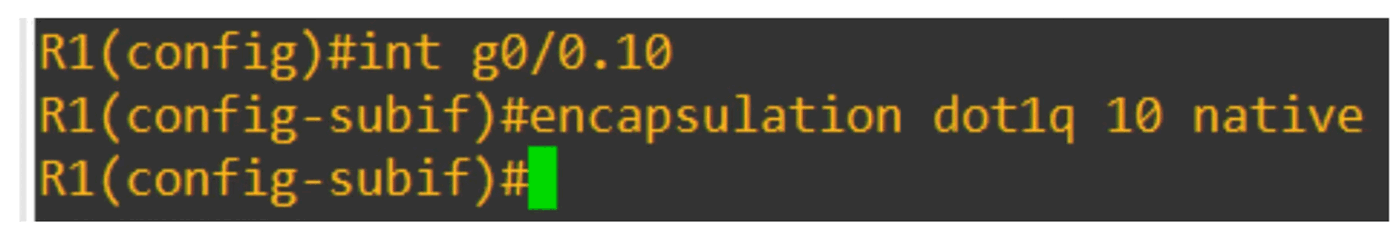
\includegraphics[keepaspectratio,alt={image}]{images/19-vlan-part3/img-003.png}}
\end{figure}

OR

\begin{itemize}
\tightlist
\item
  Configure the IP address for the native VLAN on the router's physical
  interface (the ``\textbf{encapsulation dot1q}
  \textless vlan-id\textgreater{} command is not necessary''
\end{itemize}

\begin{figure}
\centering
\pandocbounded{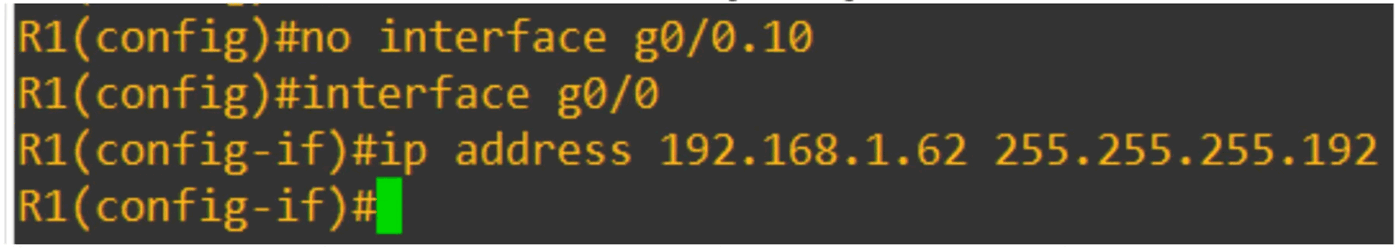
\includegraphics[keepaspectratio,alt={image}]{images/19-vlan-part3/img-004.png}}
\end{figure}

Output of ``show running-config'' of G0/0 Interface

\begin{figure}
\centering
\pandocbounded{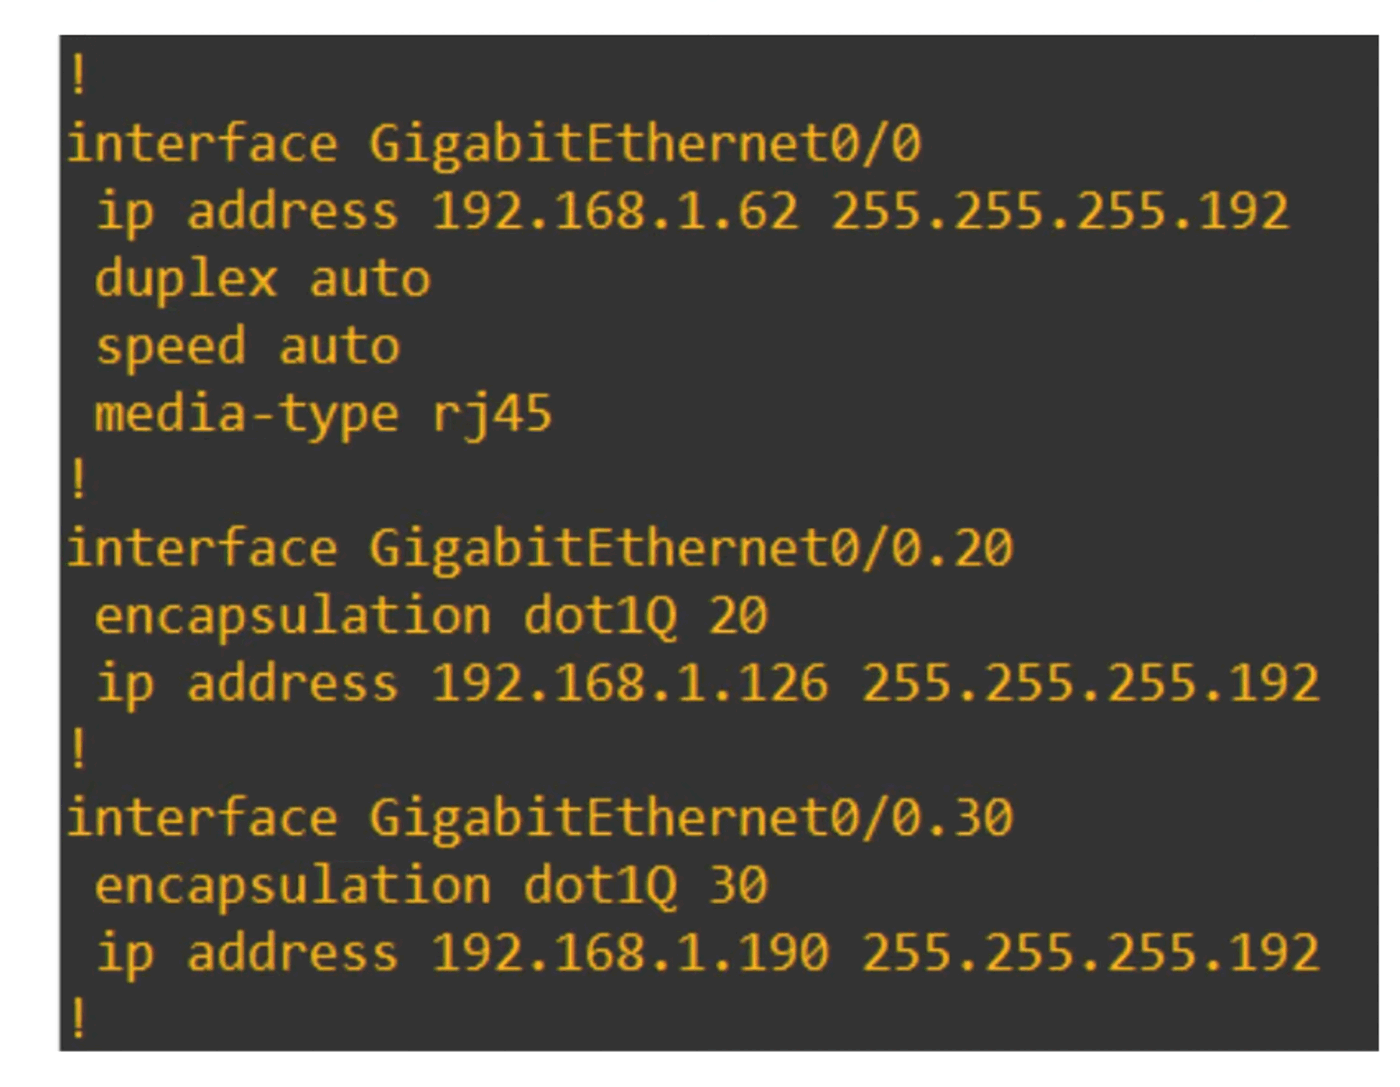
\includegraphics[keepaspectratio,alt={image}]{images/19-vlan-part3/img-005.png}}
\end{figure}

\section{Layer 3 (Multilayer)
Switches}\label{layer-3-multilayer-switches}

\section{Icon Appearance}\label{icon-appearance}

\begin{figure}
\centering
\pandocbounded{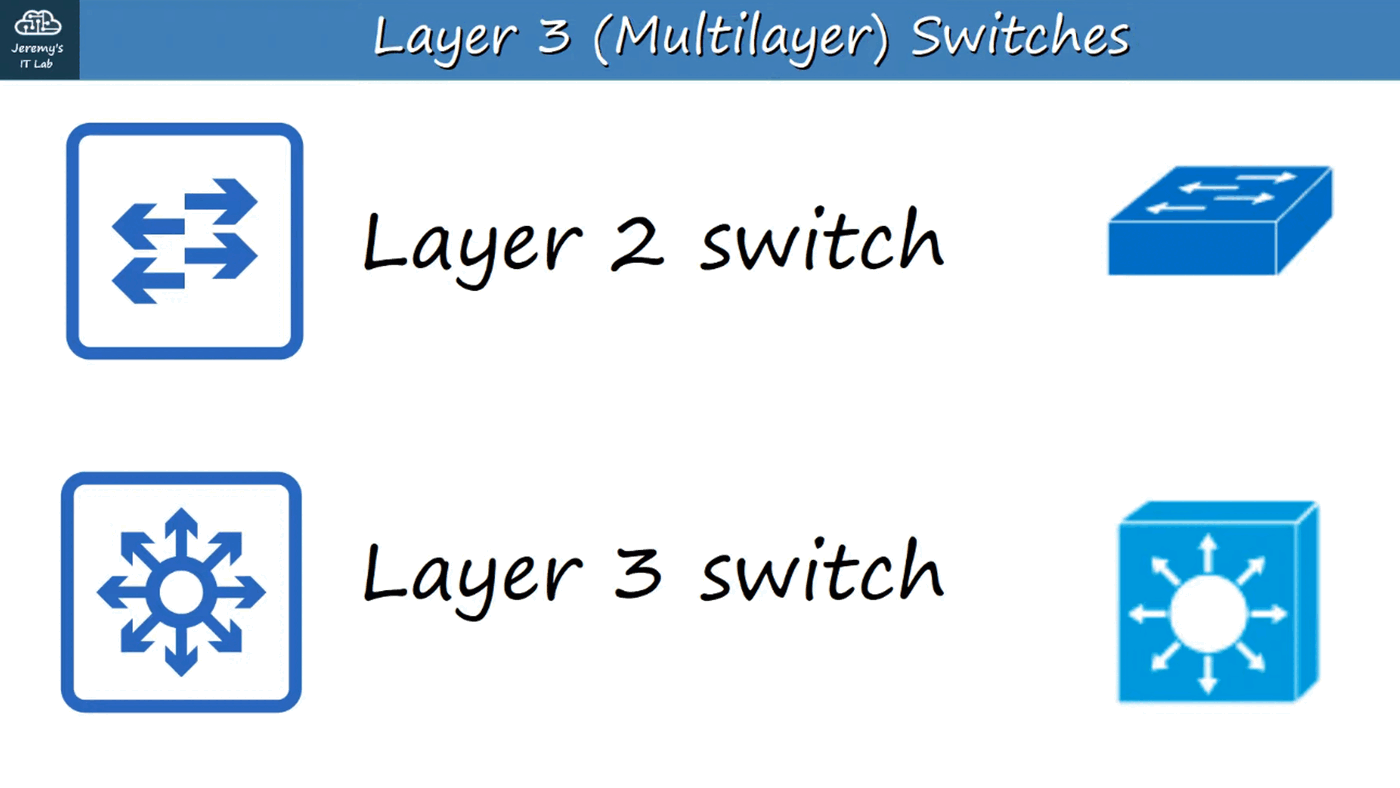
\includegraphics[keepaspectratio,alt={image}]{images/19-vlan-part3/img-006.png}}
\end{figure}

\begin{itemize}
\tightlist
\item
  A MULTILAYER SWITCH is capable of both SWITCHING and ROUTING
\item
  It is LAYER 3 AWARE
\item
  You can assign IP Addresses to its L3 Virtual Interface, like a router
\item
  You can create Virtual Interfaces for each VLAN, and assign IP
  addresses to those interfaces
\item
  You can configure routes on it, just like a ROUTER
\item
  It can be used for inter-VLAN routing
\end{itemize}

\begin{figure}
\centering
\pandocbounded{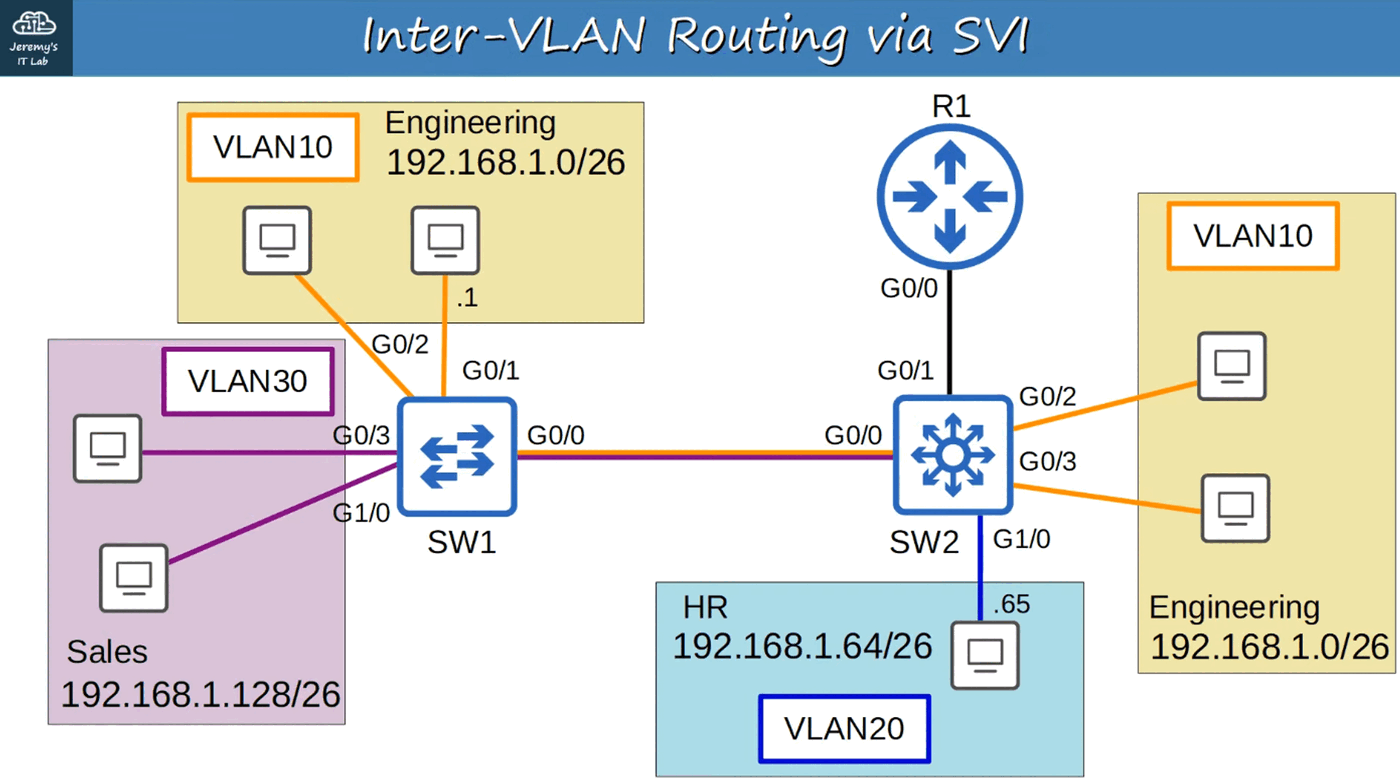
\includegraphics[keepaspectratio,alt={image}]{images/19-vlan-part3/img-007.png}}
\end{figure}

SW2 Replaced with a Layer 3 Switch

Multi-VLAN connections to R1 removed and replaced with a point-to-point
Layer 3 connection

\begin{figure}
\centering
\pandocbounded{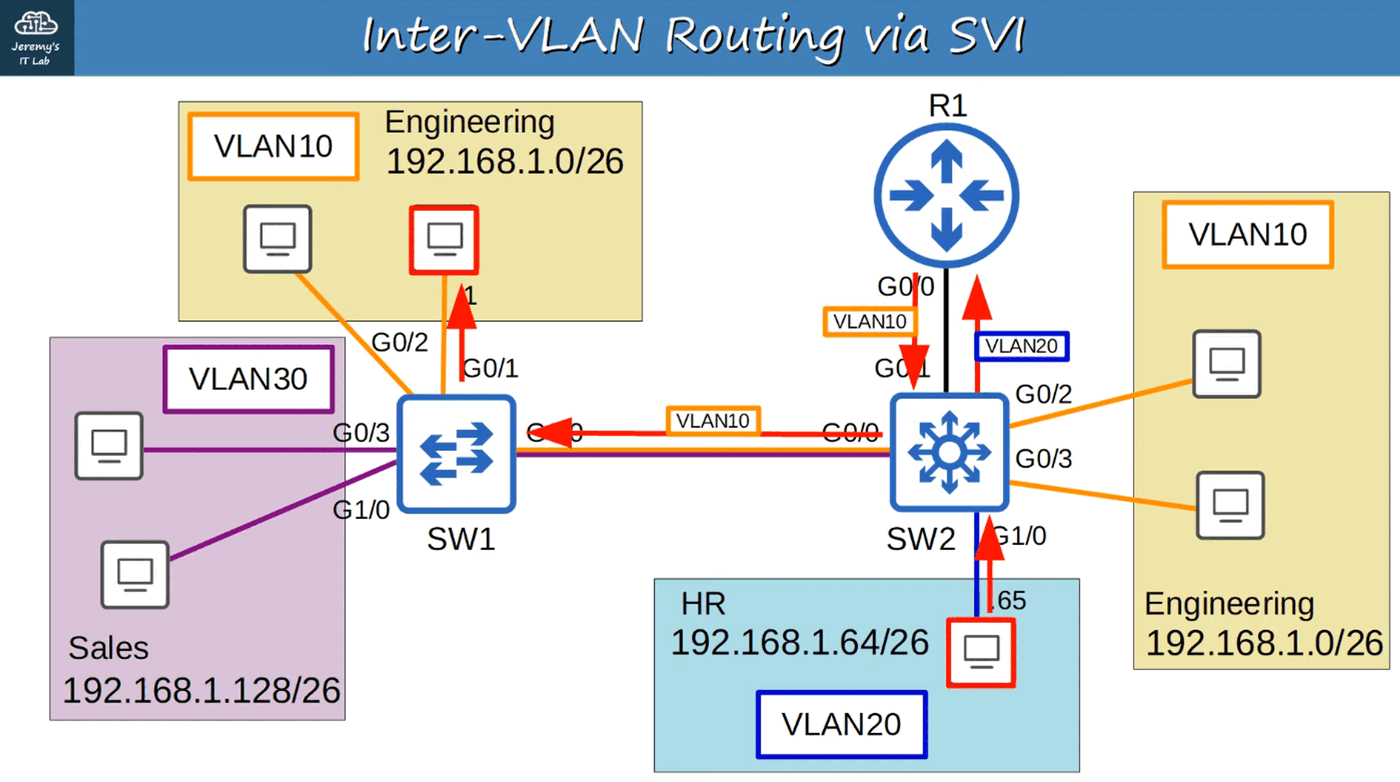
\includegraphics[keepaspectratio,alt={image}]{images/19-vlan-part3/img-008.png}}
\end{figure}

\begin{itemize}
\tightlist
\item
  SVIs (Switch Virtual Interfaces) are the virtual interfaces you can
  assign IP addresses to in a MULTILAYER SWITCH.
\item
  Configure each HOST to use the SVI (NOT the ROUTER R1) as their
  Gateway Address
\item
  To send traffic to different SUBNETS / VLANS, the PCs will send
  traffic to the SWITCH, and the SWITCH will route the traffic.
\end{itemize}

\begin{figure}
\centering
\pandocbounded{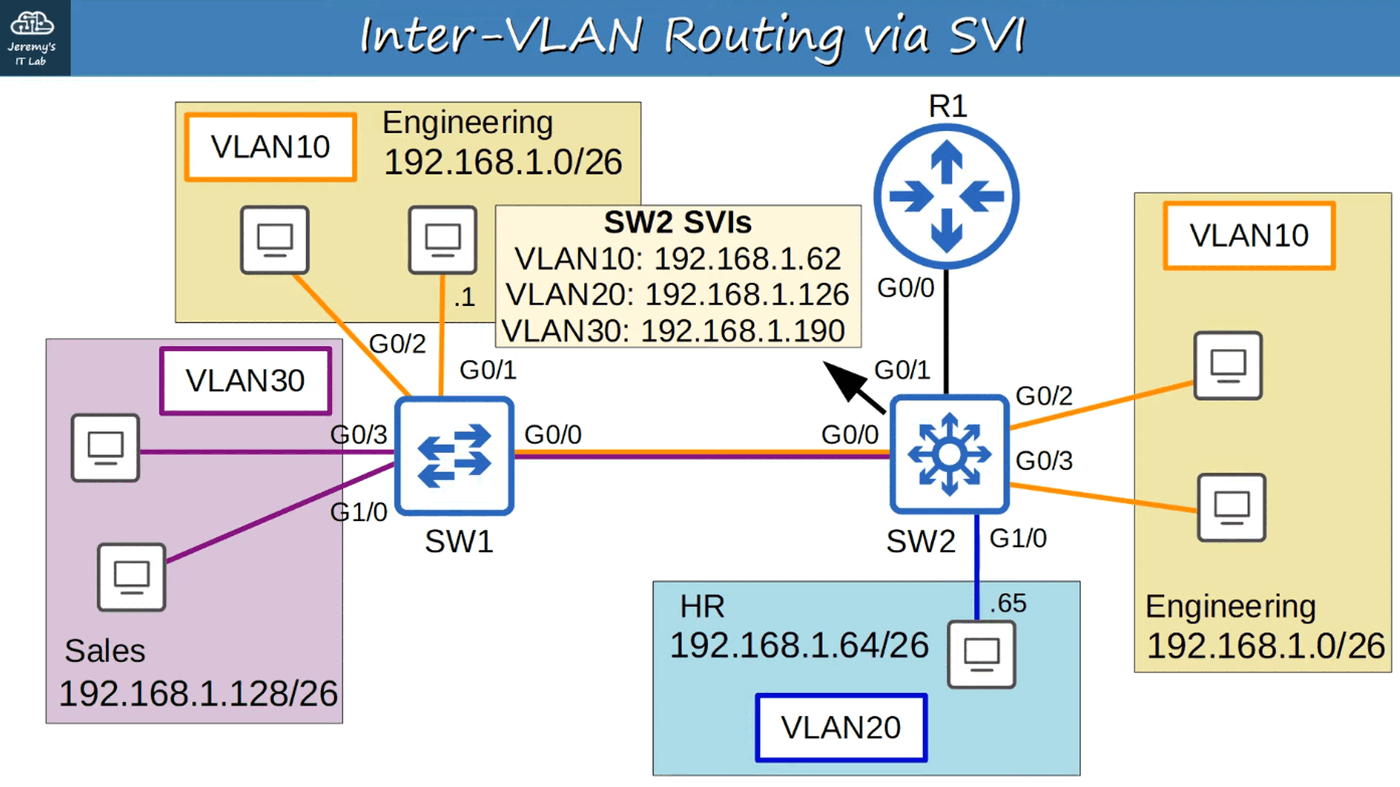
\includegraphics[keepaspectratio,alt={image}]{images/19-vlan-part3/img-009.png}}
\end{figure}

\begin{figure}
\centering
\pandocbounded{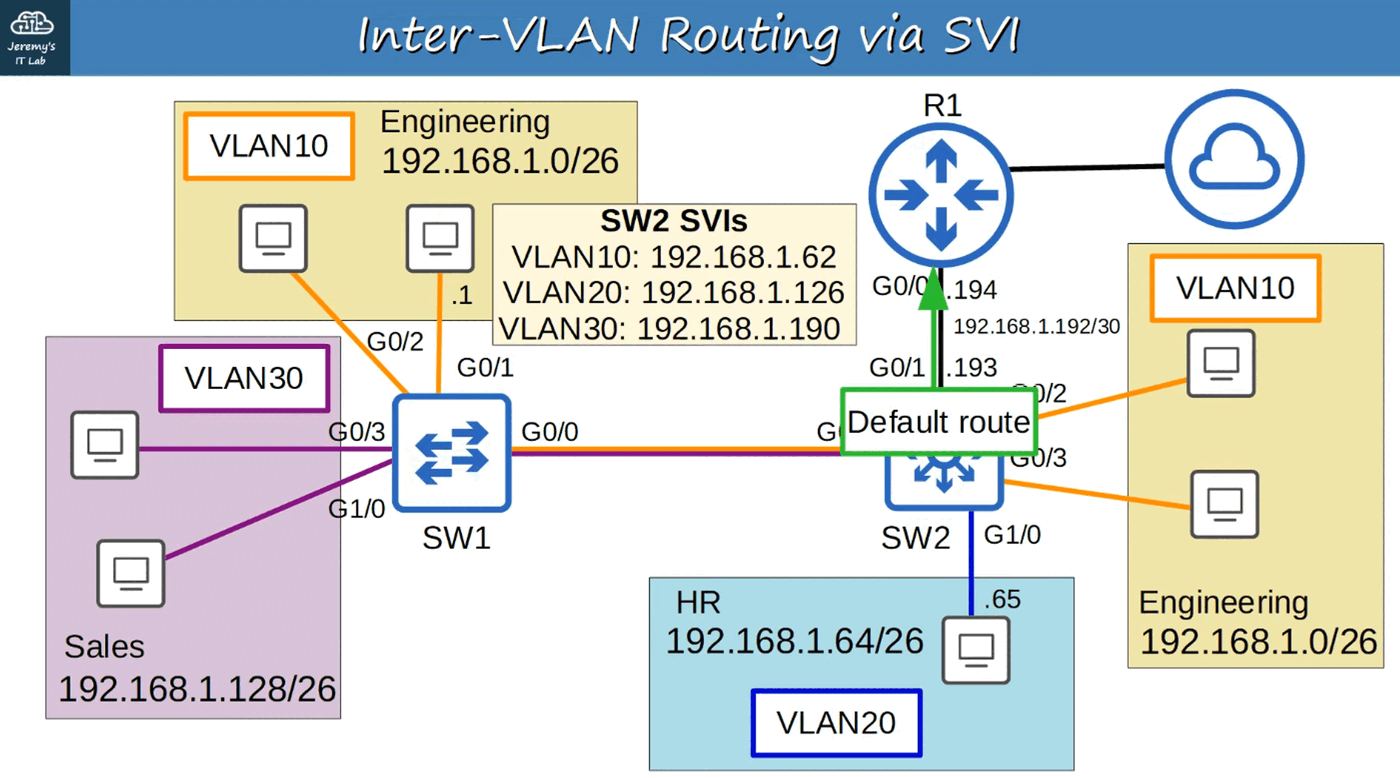
\includegraphics[keepaspectratio,alt={image}]{images/19-vlan-part3/img-010.png}}
\end{figure}

Clearing R1 configuration to set to work with the Layer 3 Point-to-Point
connection

\begin{figure}
\centering
\pandocbounded{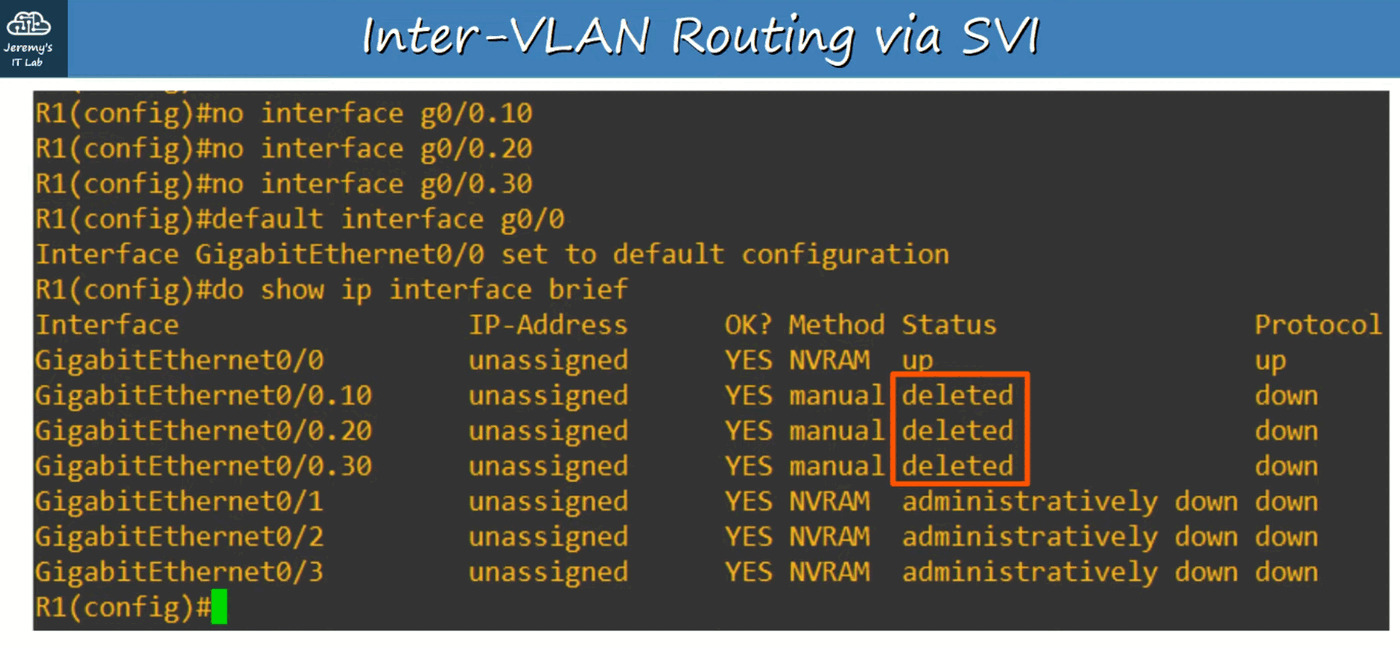
\includegraphics[keepaspectratio,alt={image}]{images/19-vlan-part3/img-011.png}}
\end{figure}

\#no interface \textless sub-interface id\textgreater{} : removes the
VLAN interface

\#default interface g0/0 : resets the g0/0 interface to it's default
settings

Then configure the default R1 G0/0 interface's to IP address :
192.168.1.194 (as per the network diagram)

Configuration of SW2 to use SVI and the Layer 3 Point-to-Point
connection with R1

\begin{figure}
\centering
\pandocbounded{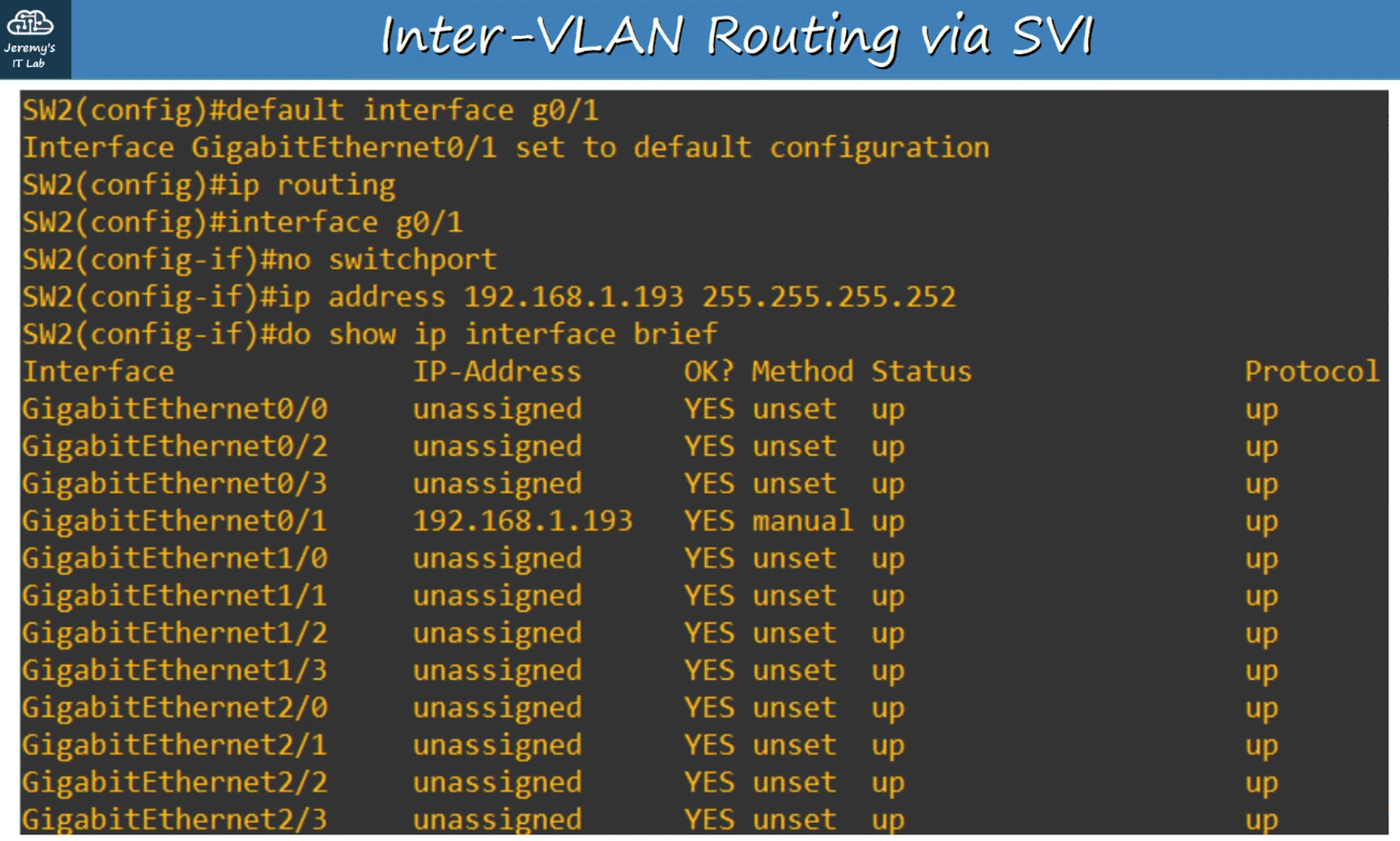
\includegraphics[keepaspectratio,alt={image}]{images/19-vlan-part3/img-012.png}}
\end{figure}

``default interface \textless interface-id\textgreater'' : resets
settings on specified interface to defaults

``ip routing'' : \textbf{IMPORTANT} command to enable Layer 3 routing on
the SWITCH

``no switchport'' : configures the interface from a Layer 2 Switchport
to a Layer 3 ``routed port''

The sets the Default Route to R1 (192.168.1.194) so that all traffic
leaving the network gets routed through R1's Gateway of Last Resort (aka
The Default Gateway)

\begin{figure}
\centering
\pandocbounded{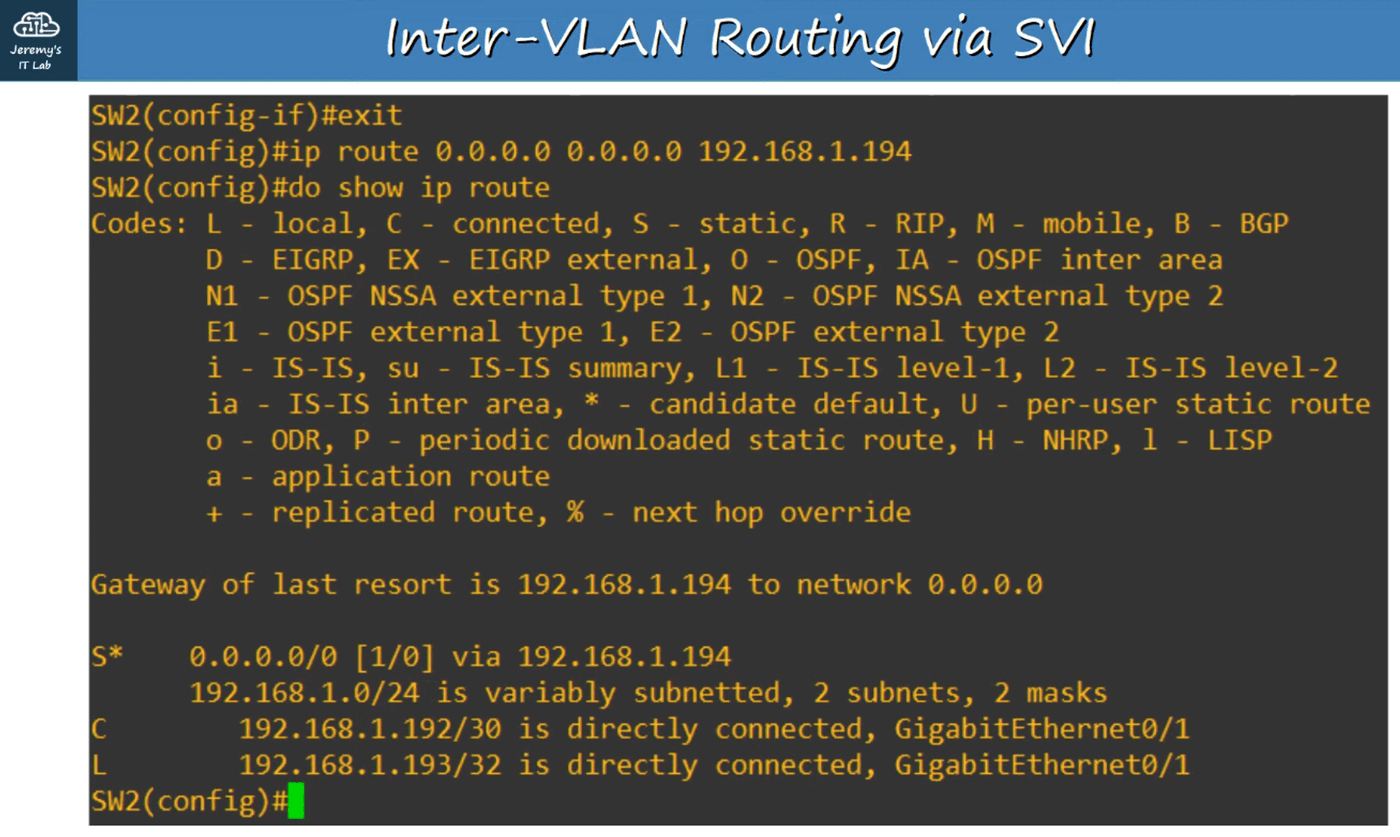
\includegraphics[keepaspectratio,alt={image}]{images/19-vlan-part3/img-013.png}}
\end{figure}

\begin{figure}
\centering
\pandocbounded{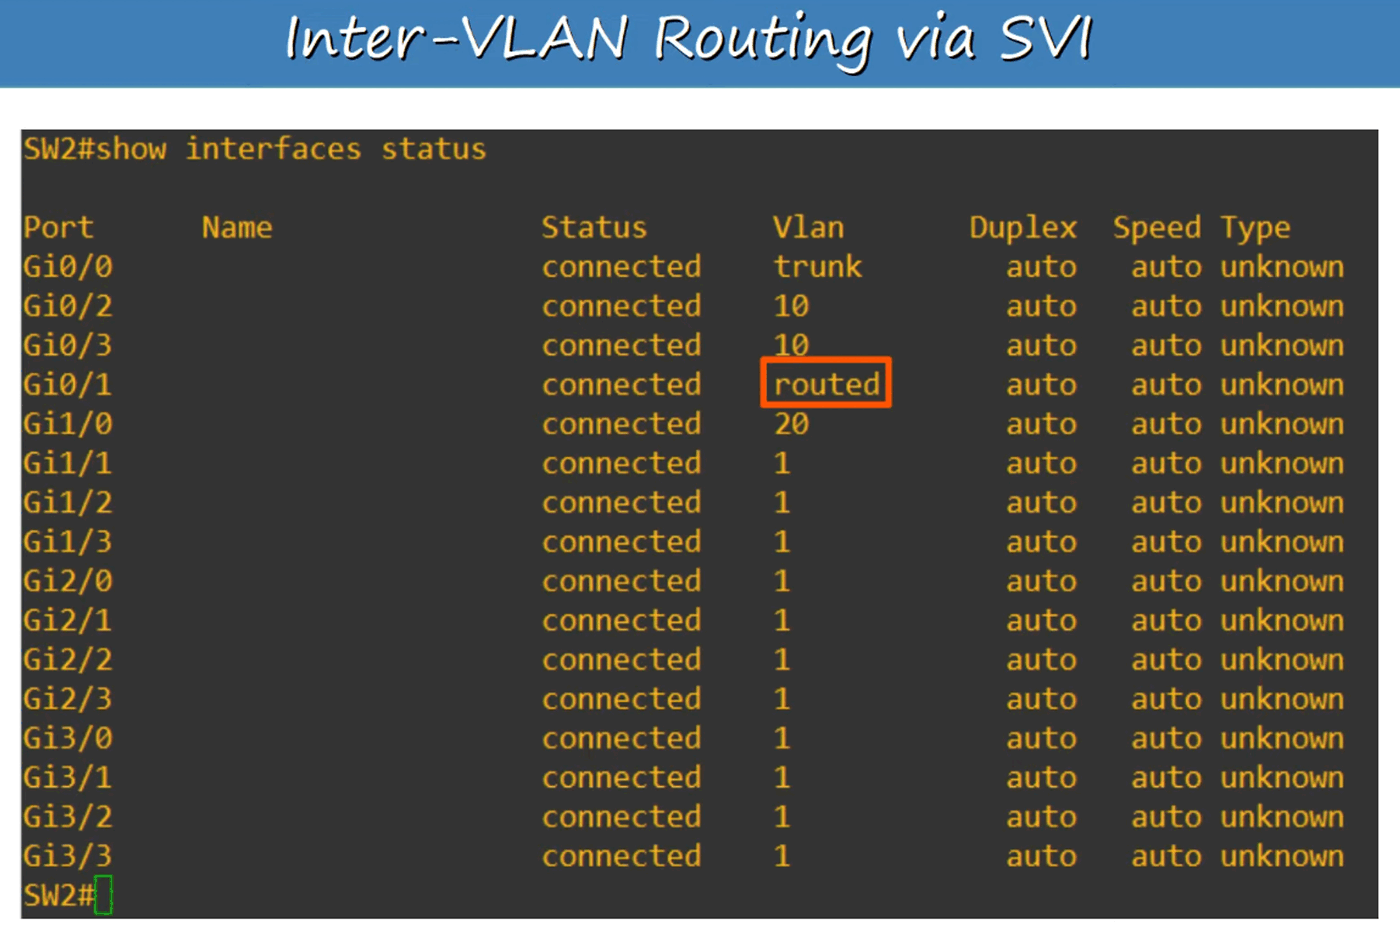
\includegraphics[keepaspectratio,alt={image}]{images/19-vlan-part3/img-014.png}}
\end{figure}

SVI CONFIGURATION ON SW2 (Virtual LAYER 3 ROUTING INTERFACES)

\begin{figure}
\centering
\pandocbounded{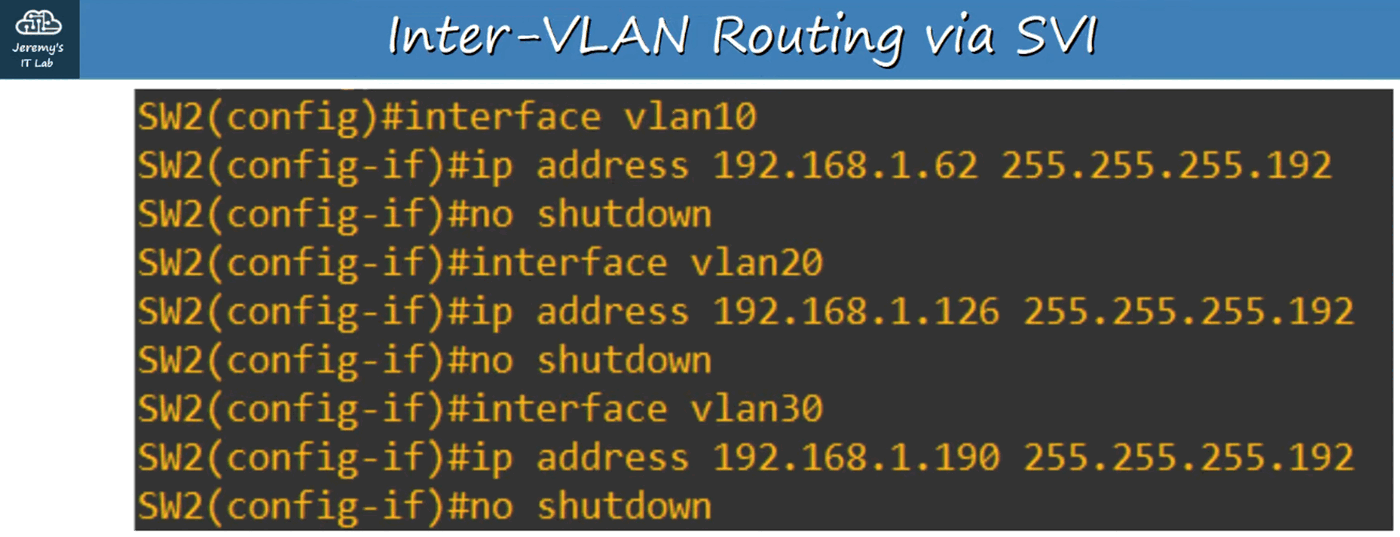
\includegraphics[keepaspectratio,alt={image}]{images/19-vlan-part3/img-015.png}}
\end{figure}

SVIs are \textbf{shut down} by default, so remember to use ``no
shutdown''

\begin{figure}
\centering
\pandocbounded{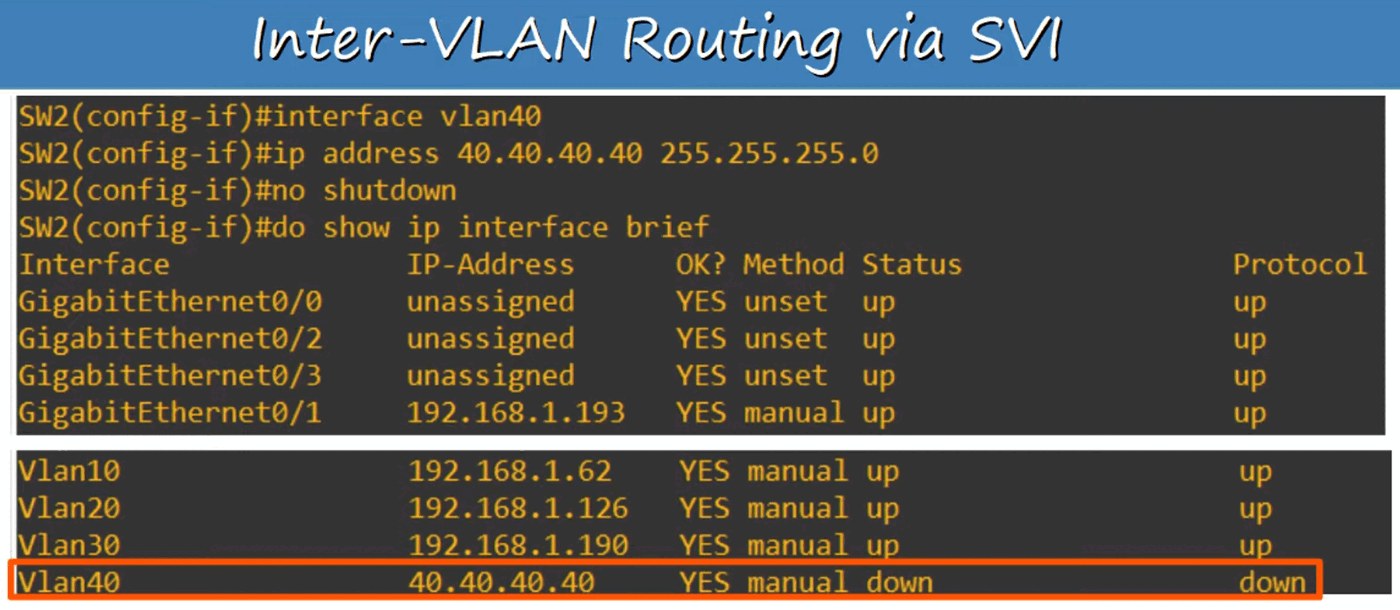
\includegraphics[keepaspectratio,alt={image}]{images/19-vlan-part3/img-016.png}}
\end{figure}

Creating an unknown SVI (VLAN 40) and the Status/Protocol is
``down/down''

What are the conditions for a SVI to be ``up/up'' ?

\begin{itemize}
\tightlist
\item
  The VLAN must exist on the SWITCH
\item
  The SWITCH must have at least ONE access port in the VLAN in an
  ``up/up'' state AND/OR one TRUNK port that allows the VLAN that is in
  an ``up/up'' state
\item
  The VLAN must not be shutdown (you can use the ``shutdown'' command to
  disable a VLAN)
\item
  The SVI must not be shutdown (SVIs are disabled, by default)
\end{itemize}

\begin{figure}
\centering
\pandocbounded{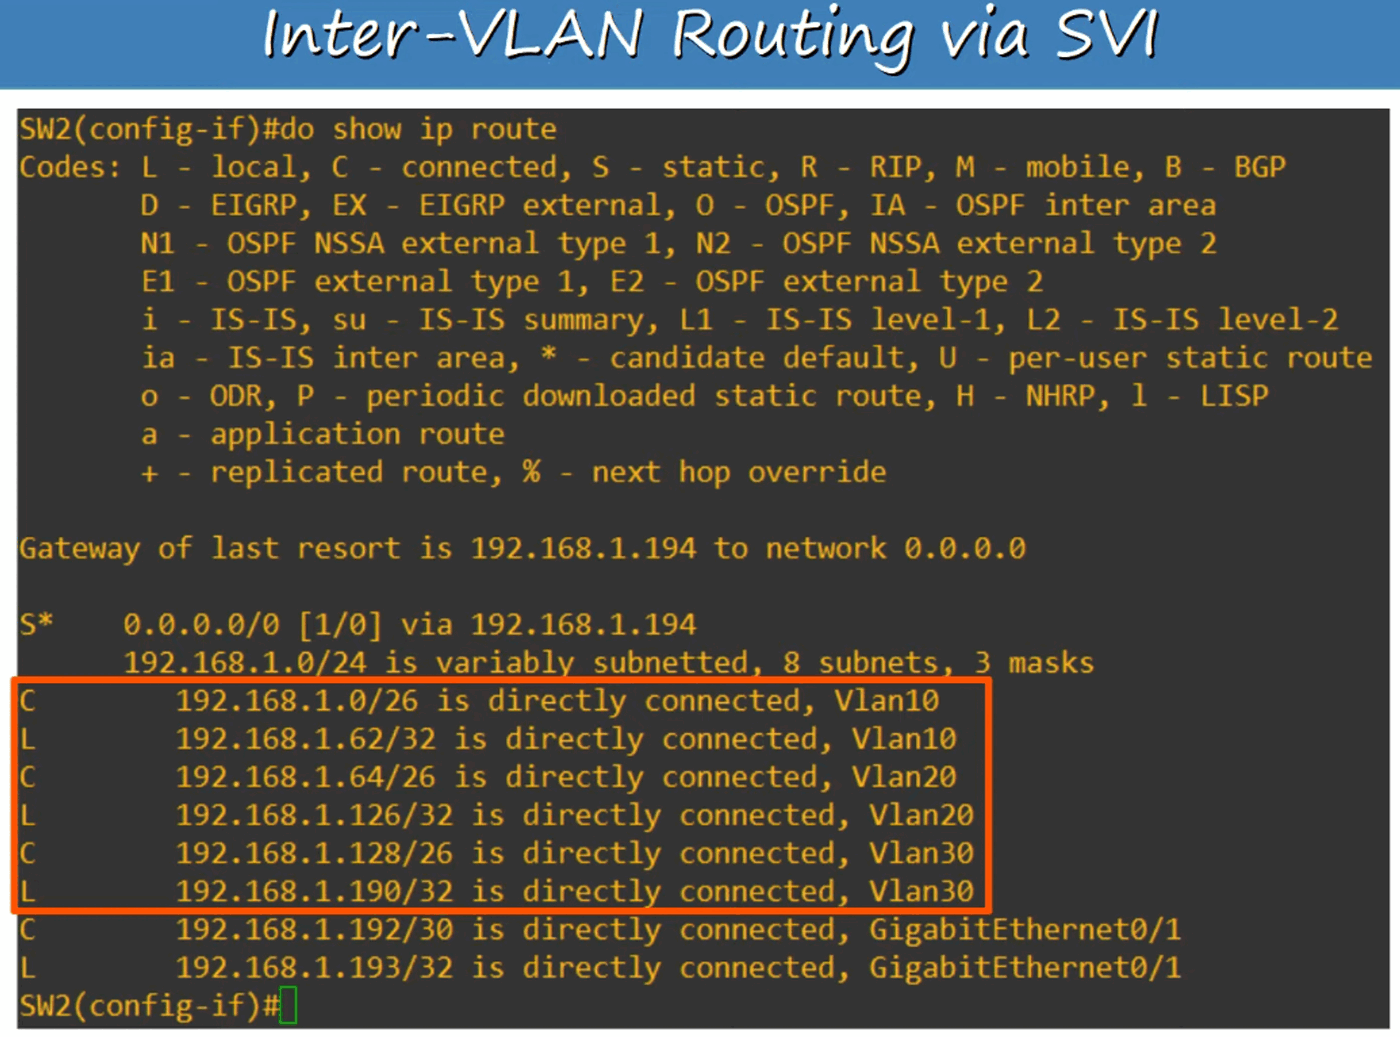
\includegraphics[keepaspectratio,alt={image}]{images/19-vlan-part3/img-017.png}}
\end{figure}

The VLAN trunk has been successfully replaced by an Layer 3 SWITCH SVI.

All hosts should be able to connect with each other (tested with
``ping'') as well as reach the external internet (via the Cloud symbol
attached to R1)
